\documentclass[12pt,a4paper]{article}
\usepackage[a4paper,top=1.5cm, bottom=1.5cm, left=1.5cm, right=1.5cm]{geometry}
\usepackage[T2A]{fontenc}
\usepackage[utf8]{inputenc}
\usepackage[russian]{babel}
\usepackage{amsmath}
\usepackage{amssymb}
\usepackage{graphicx}
\usepackage{floatrow}
\usepackage{booktabs}
\usepackage{wrapfig}
\usepackage{indentfirst}
\usepackage{lipsum}
\usepackage{subcaption}
\usepackage{float}
\usepackage{enumitem}
\restylefloat{table}

\newcommand{\figref}[1]{(см. рис. \ref{#1})}
\newcommand{\e}[1]{\text{$\cdot10^{#1}$}}

\title{Работа №25\\ Лестничные фильтры}
\author{Симанкович Александр \\ Б01-104}
\date{\today}

\begin{document}
	\maketitle	
	
	\subsection*{2. Активные звенья с двойным Т-мостом}
	
	Изучим АЧХ и ФЧХ полосового фильтра.

	\begin{figure}[H]
		\centering
		\begin{minipage}[b]{.5\textwidth}
			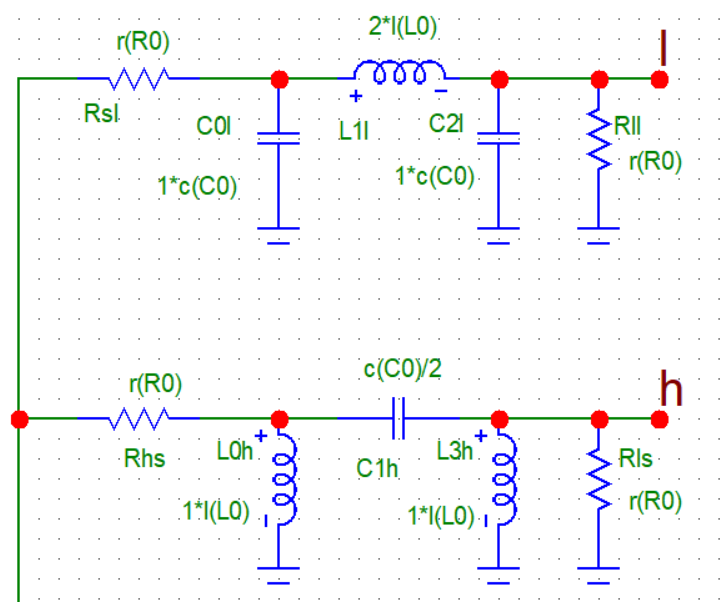
\includegraphics[width=0.9\linewidth]{res/adm3p_lh.png}
		\end{minipage}%
		\begin{minipage}[b]{.5\textwidth}
			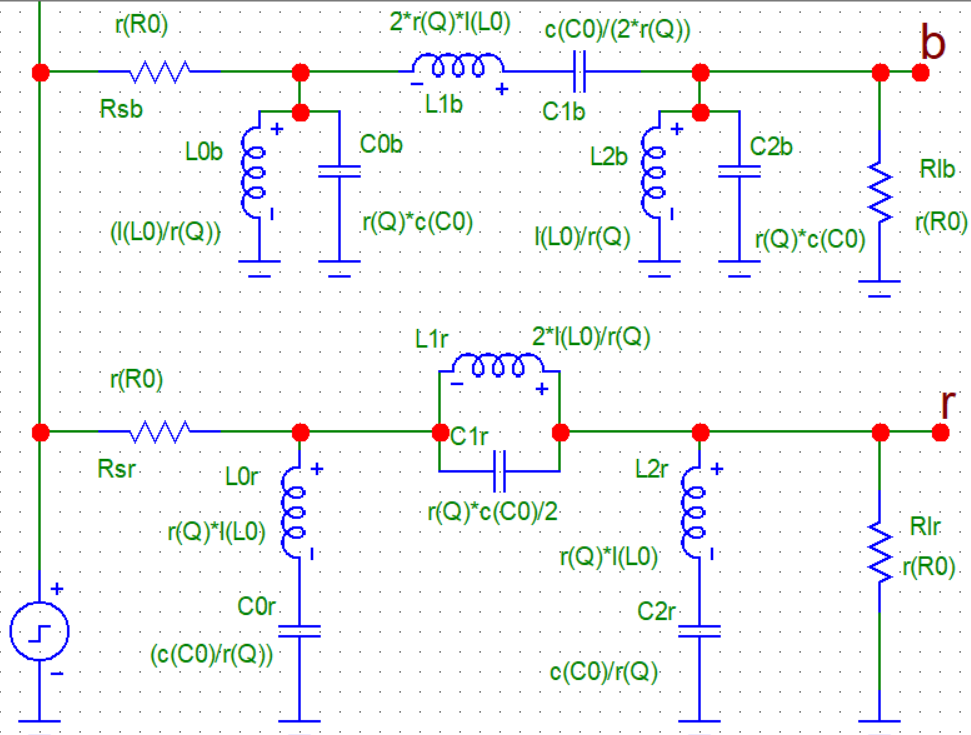
\includegraphics[width=0.9\linewidth]{res/adm3p_br.png}
		\end{minipage}
		\caption*{Схемы ФНЧ, ФВЧ, ПФ, РФ через адмиттанс}
	\end{figure}

	\begin{figure}[H]
		\centering
		\begin{minipage}[b]{.5\textwidth}
			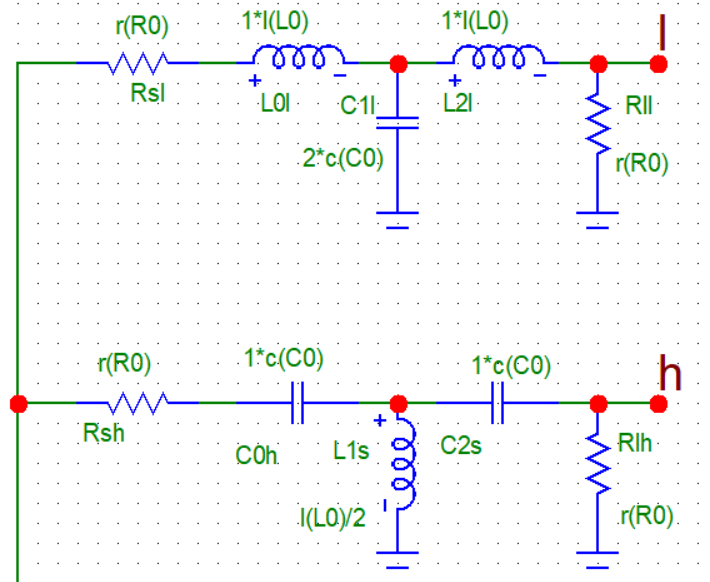
\includegraphics[width=0.9\linewidth]{res/imp3p_lh.png}
		\end{minipage}%
		\begin{minipage}[b]{.5\textwidth}
			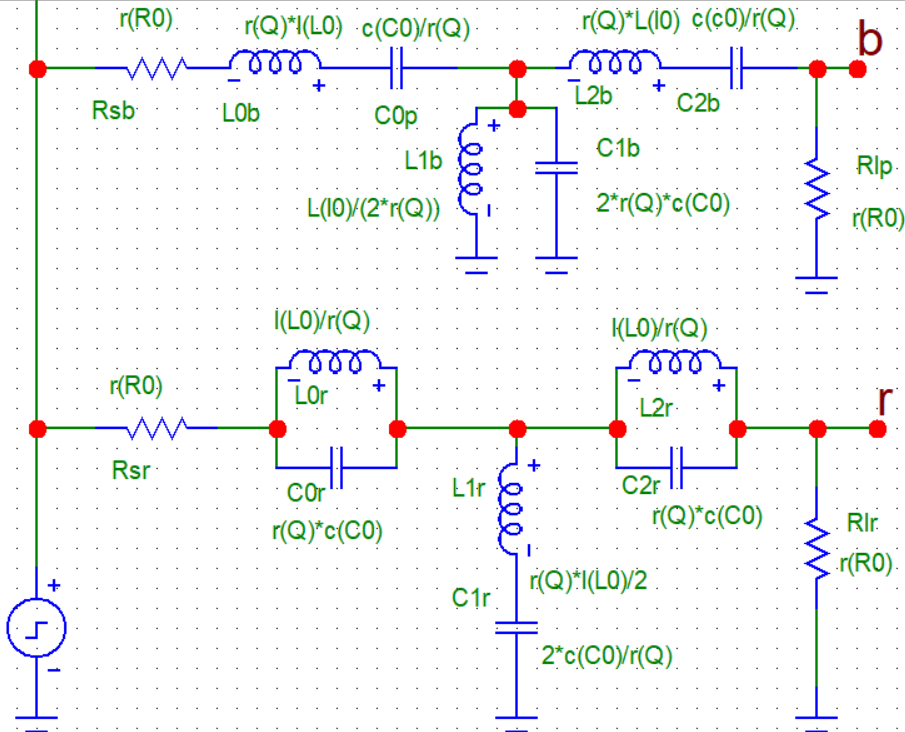
\includegraphics[width=0.9\linewidth]{res/imp3p_br.png}
		\end{minipage}
		\caption*{Схемы ФНЧ, ФВЧ, ПФ, РФ через импеданс}
	\end{figure}

	Приведем графики АЧХ для фильтров.

	\begin{figure}[H]
		\centering
		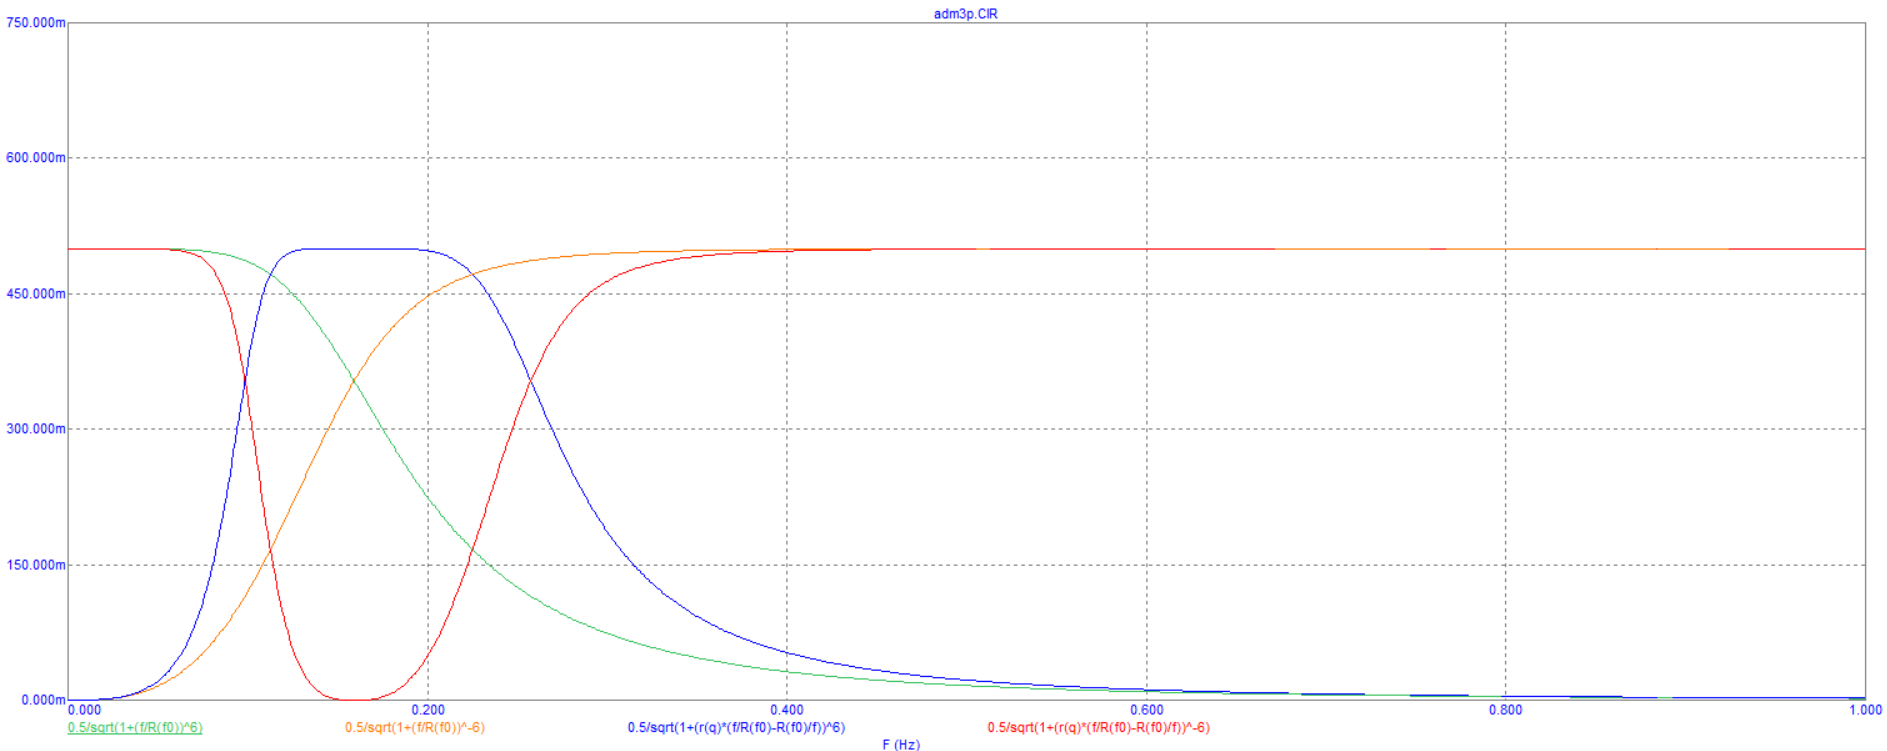
\includegraphics[width=1.0\linewidth]{res/adm3p_ach.png}
		\caption{АЧХ фильтров}
		\label{ach}
	\end{figure}
	
	\subsection*{9.2 Трехполюсные лестничные фильтры}
	
	\subsubsection*{1}
	Реализуем лестничные фильтры через импеданс.
	
	Параметры фильтра: $R_0 = 50,\; f_0 = 1 \; MHz, \; Q = 10$.
	
	Вычислим параметры $L_0 = \frac{R_0}{2 \pi f_0} = 8$ мкГн, $C_0 = \frac{1}{2 \pi f_0 R_0} = 3.2$ нФ.

	\subsubsection*{2}

	\begin{figure}[H]
		\centering
		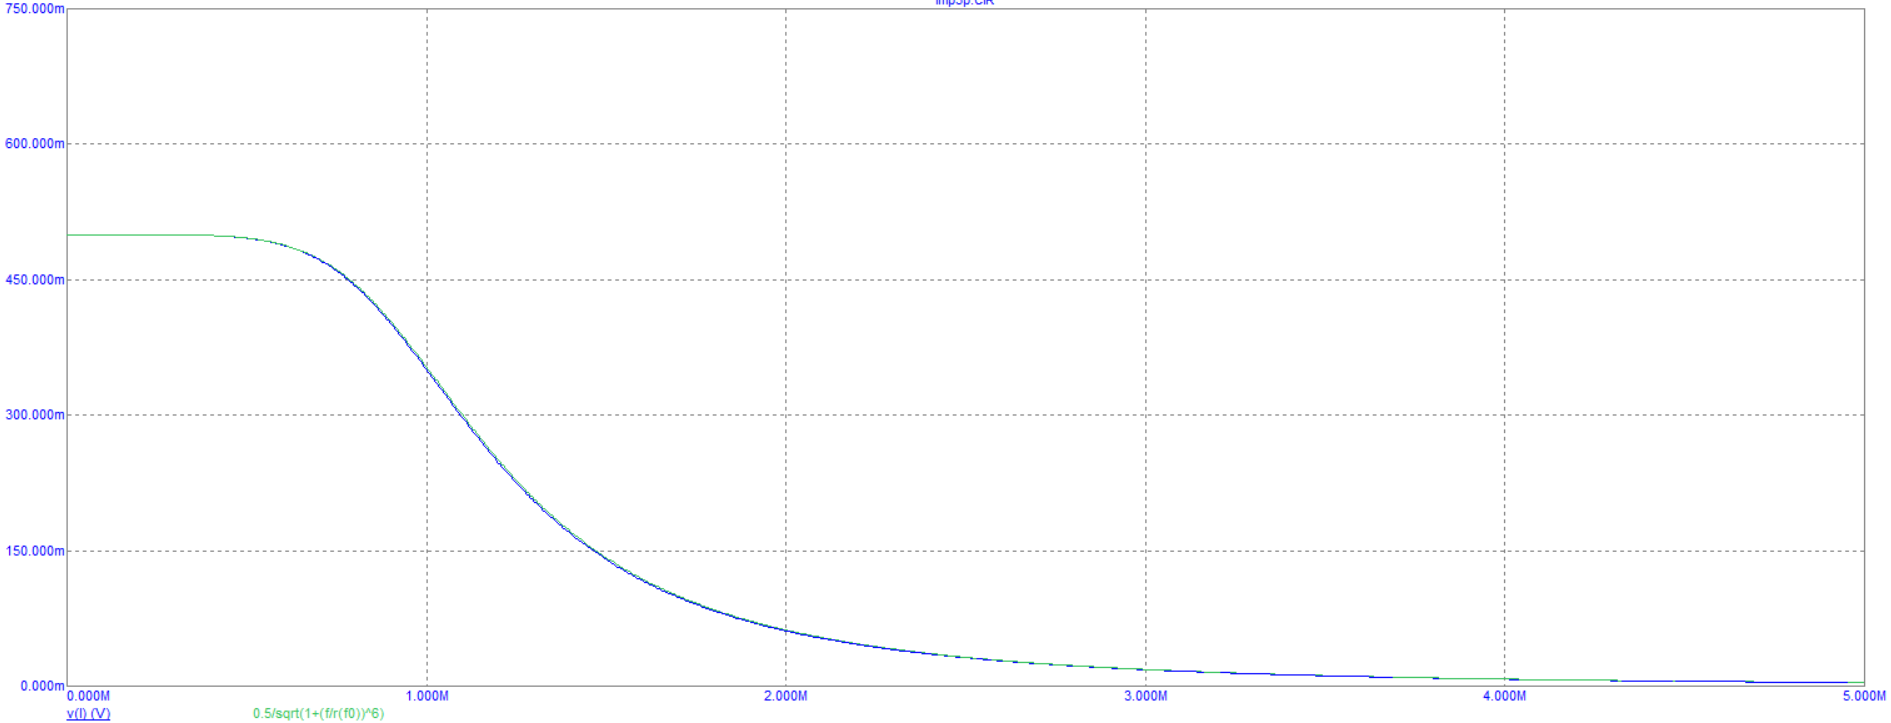
\includegraphics[width=1.0\linewidth]{res/imp3p_th.png}
		\caption{Сравнение с теорией ФНЧ}
		\label{th}
	\end{figure}

	\begin{figure}[H]
		\centering
		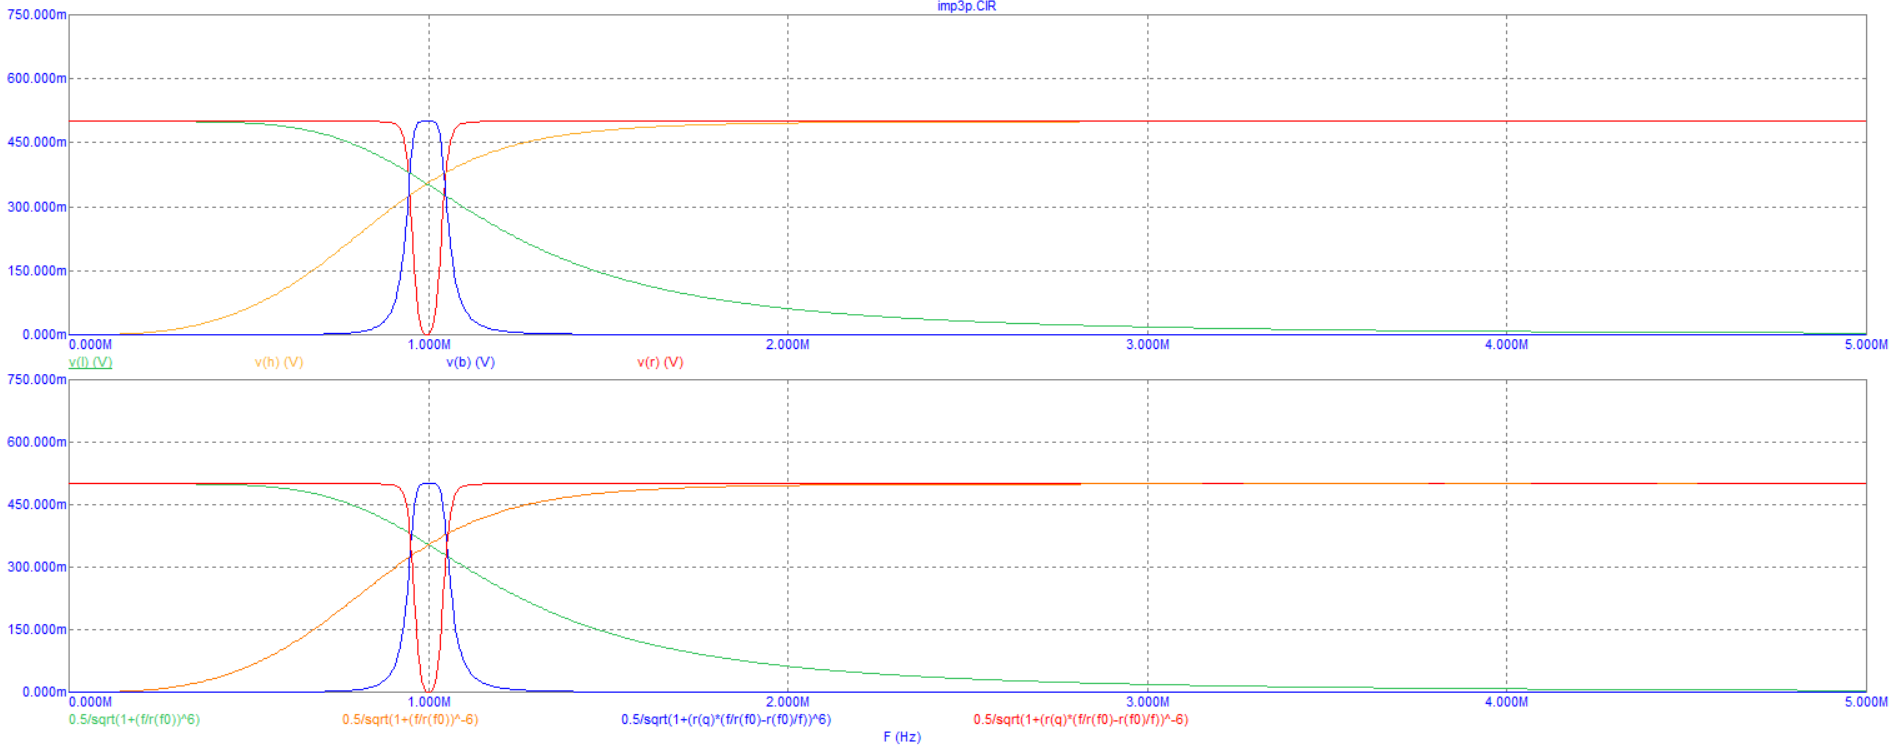
\includegraphics[width=1.0\linewidth]{res/imp3p_thall.png}
		\caption{Сравнение с теорией, все}
		\label{thall}
	\end{figure}

	\subsubsection*{3}

	Проварьируем $RLL$ и $RSL$.

	\begin{figure}[H]
		\centering
		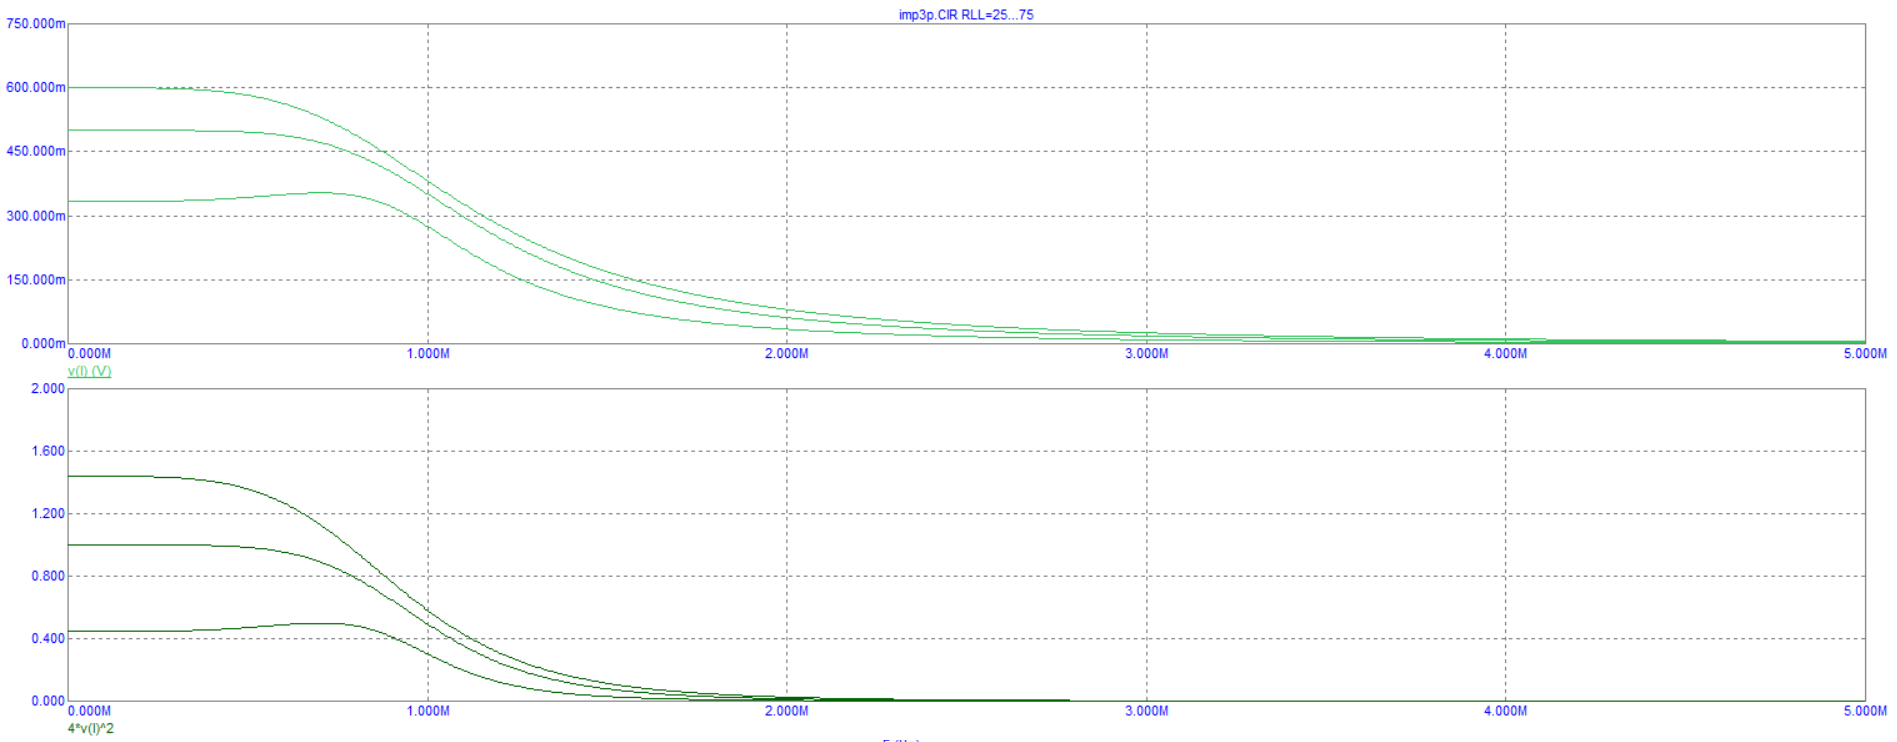
\includegraphics[width=1.0\linewidth]{res/imp3p_RLL.png}
		\caption{ФНЧ, вариация $RLL$}
		\label{rllrsl}
	\end{figure}
	
	\begin{figure}[H]
		\centering
		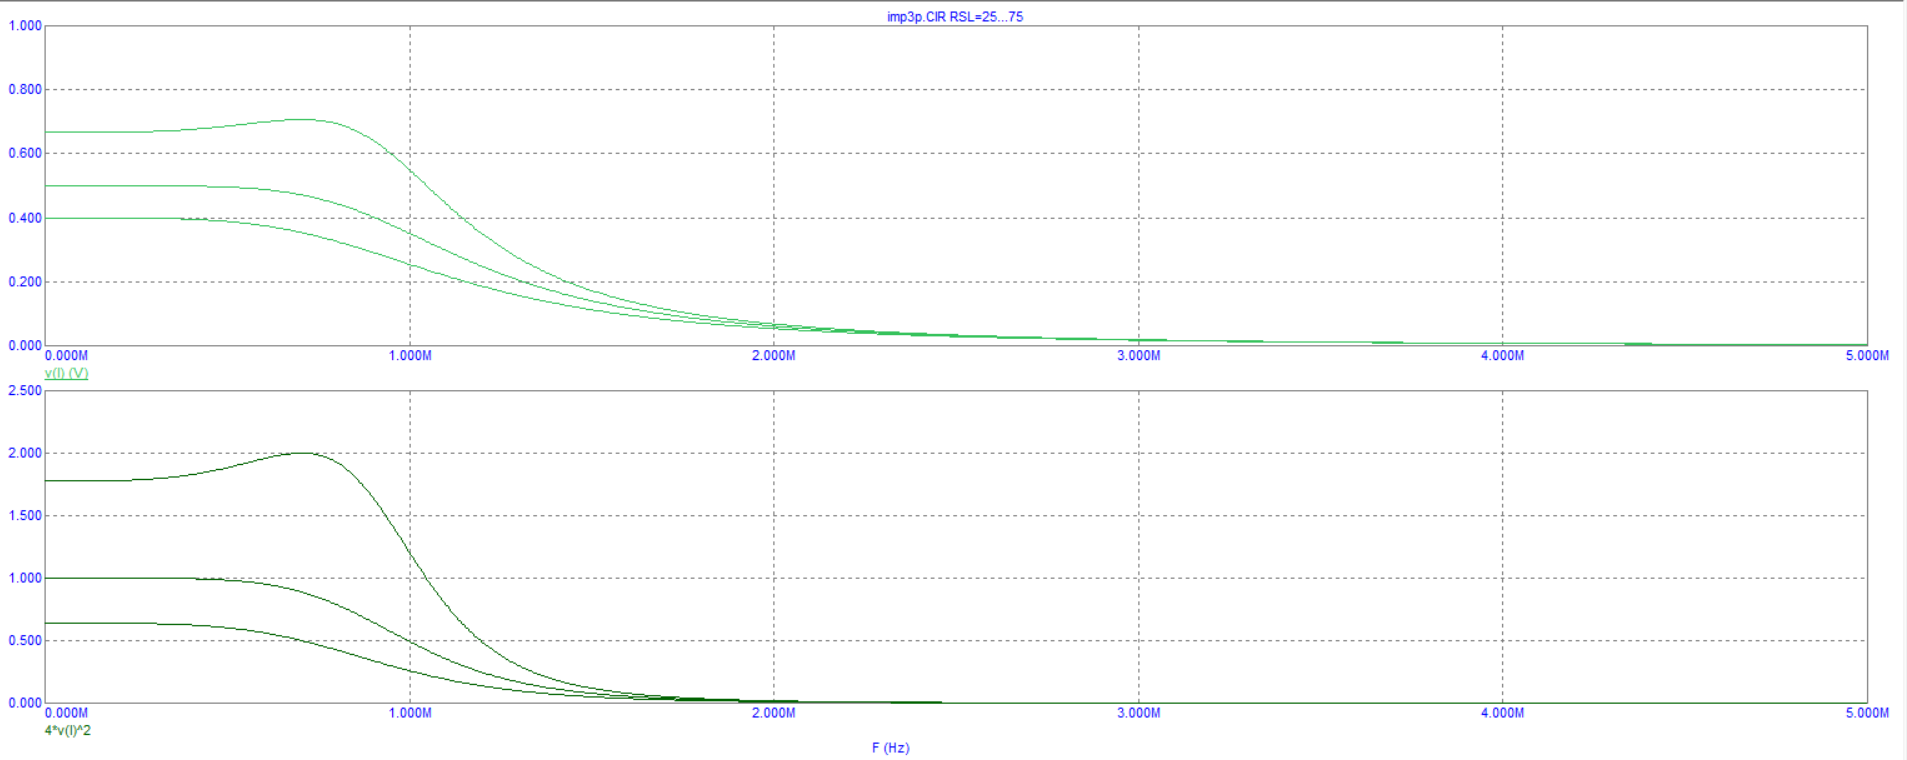
\includegraphics[width=1.0\linewidth]{res/imp3p_RSL.png}
		\caption{ФНЧ, вариация $RSL$}
		\label{rllrsl}
	\end{figure}
	
	

	Мы видим, что при повышении сопротивления фильтр "деградирует".

	\begin{table}[H]
		\begin{tabular}{llll}
			\hline
			$R_s$ & 25   & 50   & 75   \\ \hline
			$|K|$ & 0.66 & 0.50  & 0.40  \\
			$G$   & 0.89 & 1.00 & 0.96 \\ \hline
		\end{tabular}
		\caption{Деградация при варьировании $R_s$}
	\end{table}
	
	\begin{table}[H]
		\begin{tabular}{llll}
			\hline
			$R_l$ & 25   & 50   & 75   \\ \hline
			$|K|$ & 0.33 & 0.50  & 0.60  \\
			$G$   & 0.88 & 1.00 & 0.96 \\ \hline
		\end{tabular}
		\caption{Деградация при варьировании $R_l$}
	\end{table}

	\subsubsection*{4}

	Определим ФЧХ фильтров.
	
	\begin{figure}[H]
		\centering
		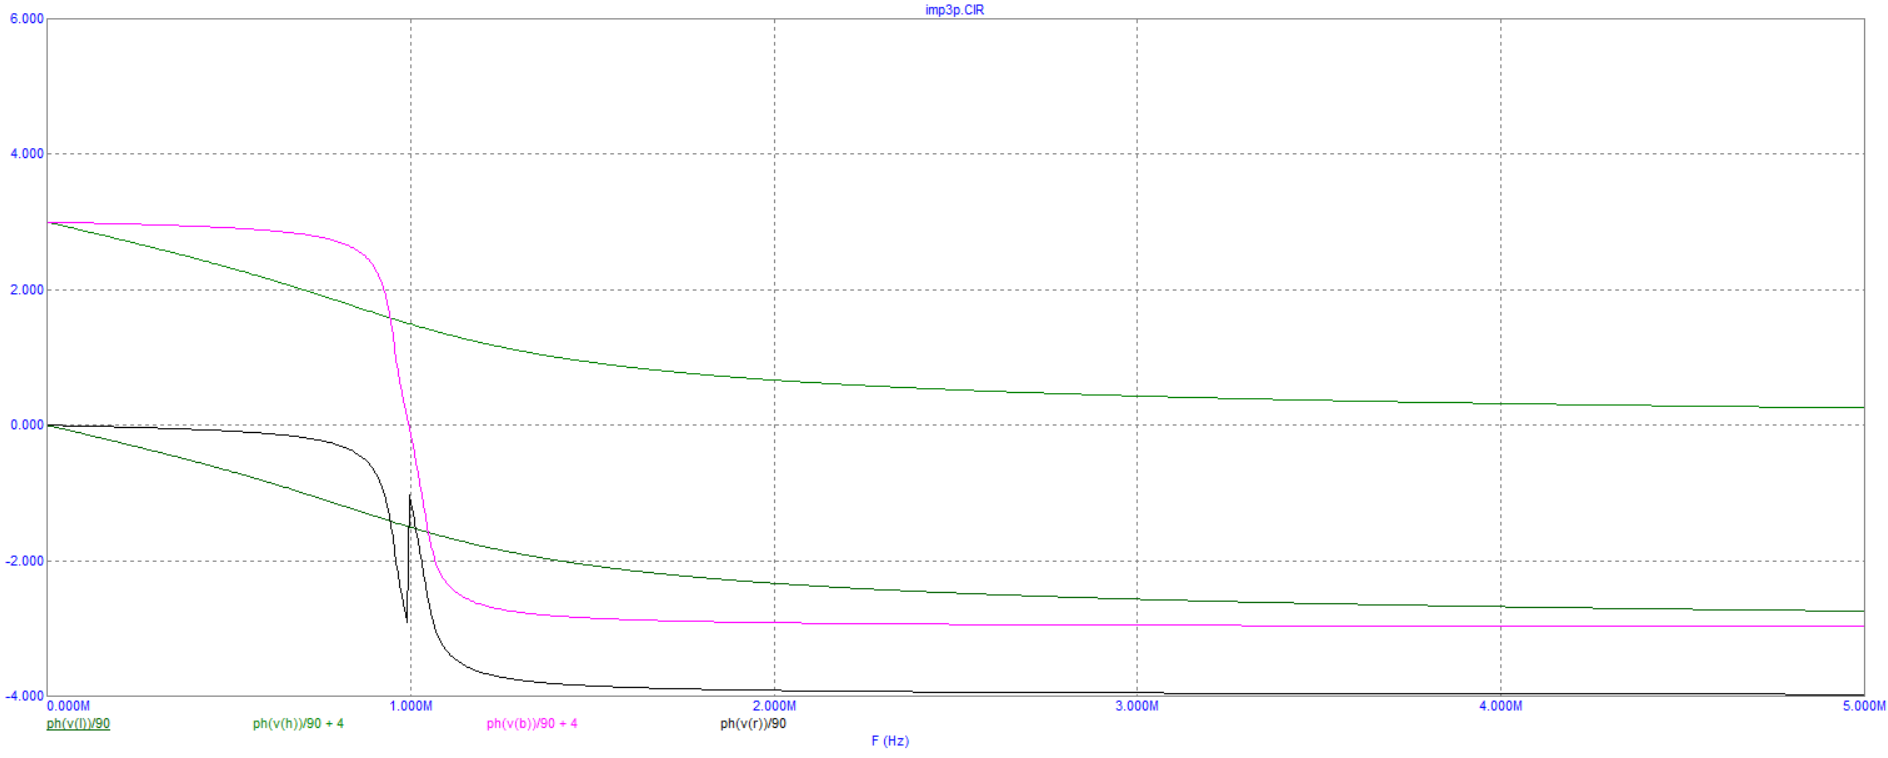
\includegraphics[width=1.0\linewidth]{res/imp3p_phase.png}
		\caption{ФЧХ}
		\label{phase}
	\end{figure}

	\begin{table}[H]
		\begin{tabular}{lllll}
			\hline
			Тип                & ФНЧ             & ФВЧ            & ПФ              & РФ              \\ \hline
			$\varphi_0$        & $0$             & $270 ^{\circ}$ & $270 ^{\circ}$  & 0               \\
			$\varphi_{\infty}$ & $-270 ^{\circ}$ & 0              & $-270 ^{\circ}$ & $-360 ^{\circ}$ \\ \hline
		\end{tabular}
	\end{table}

	\subsubsection*{5}
	
	Рассмотрим частотную характеристику ФНЧ, укажем на ней уровни затухания на $0$, $f_0$, $2f_0$, $10f_0$.

	\begin{figure}[H]
		\centering
		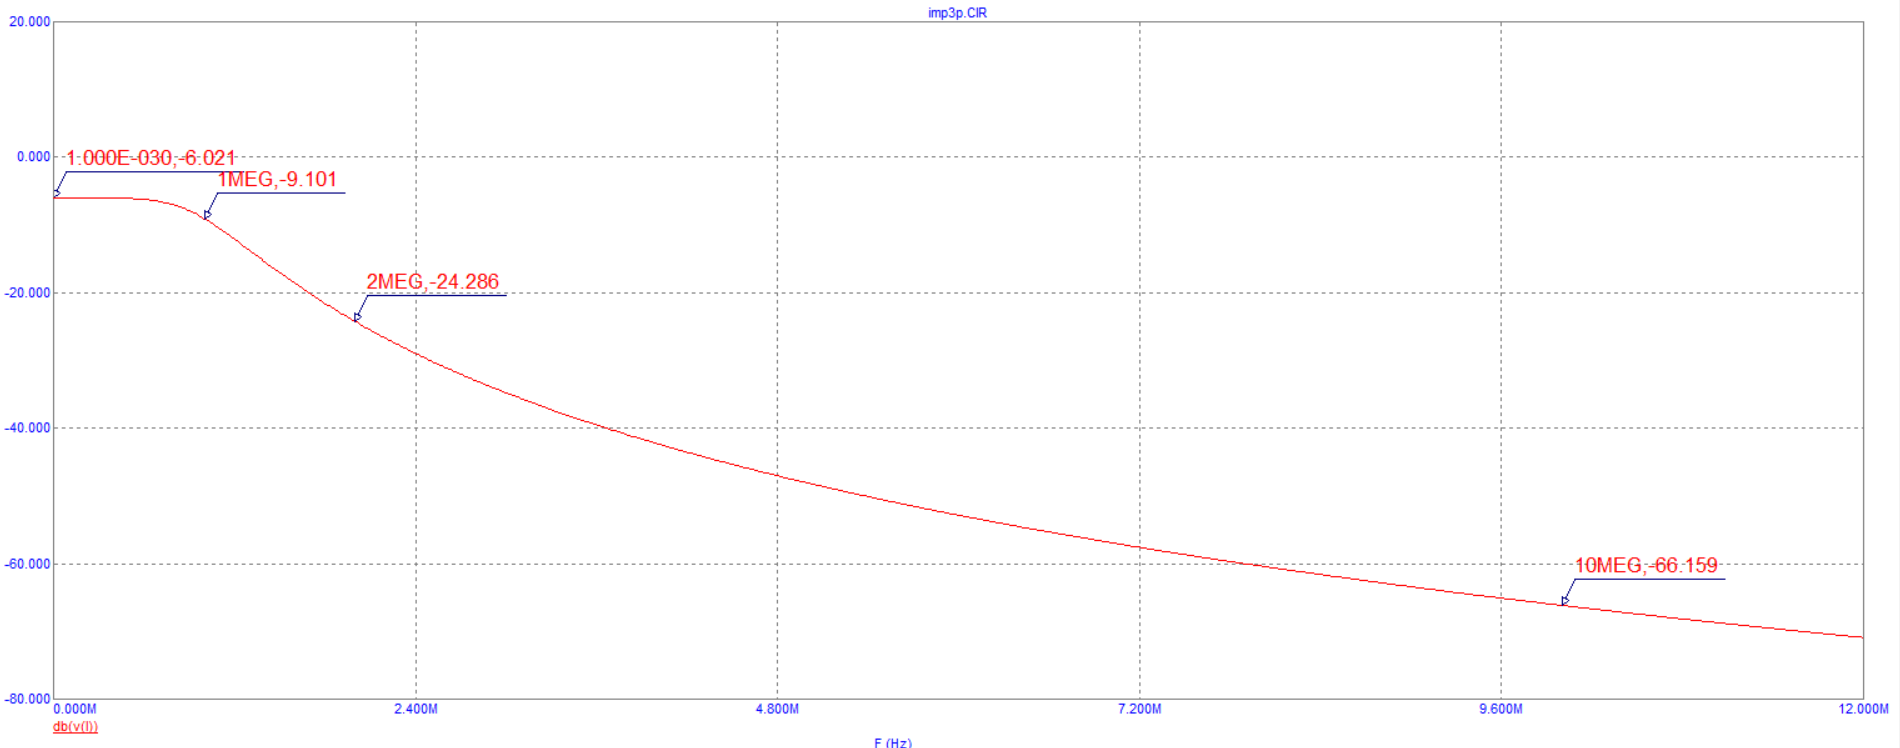
\includegraphics[width=1.0\linewidth]{res/imp3p_low_log.png}
		\caption{ФНЧ, затухание}
		\label{phase}
	\end{figure}

	\subsubsection*{6}

	Аналогично, частотную характеристику ПФ. Отобразим полосу пропускания $\Delta f$ и затухание на $2\Delta f$ и $10 \Delta f$.

	\begin{figure}[H]
		\centering
		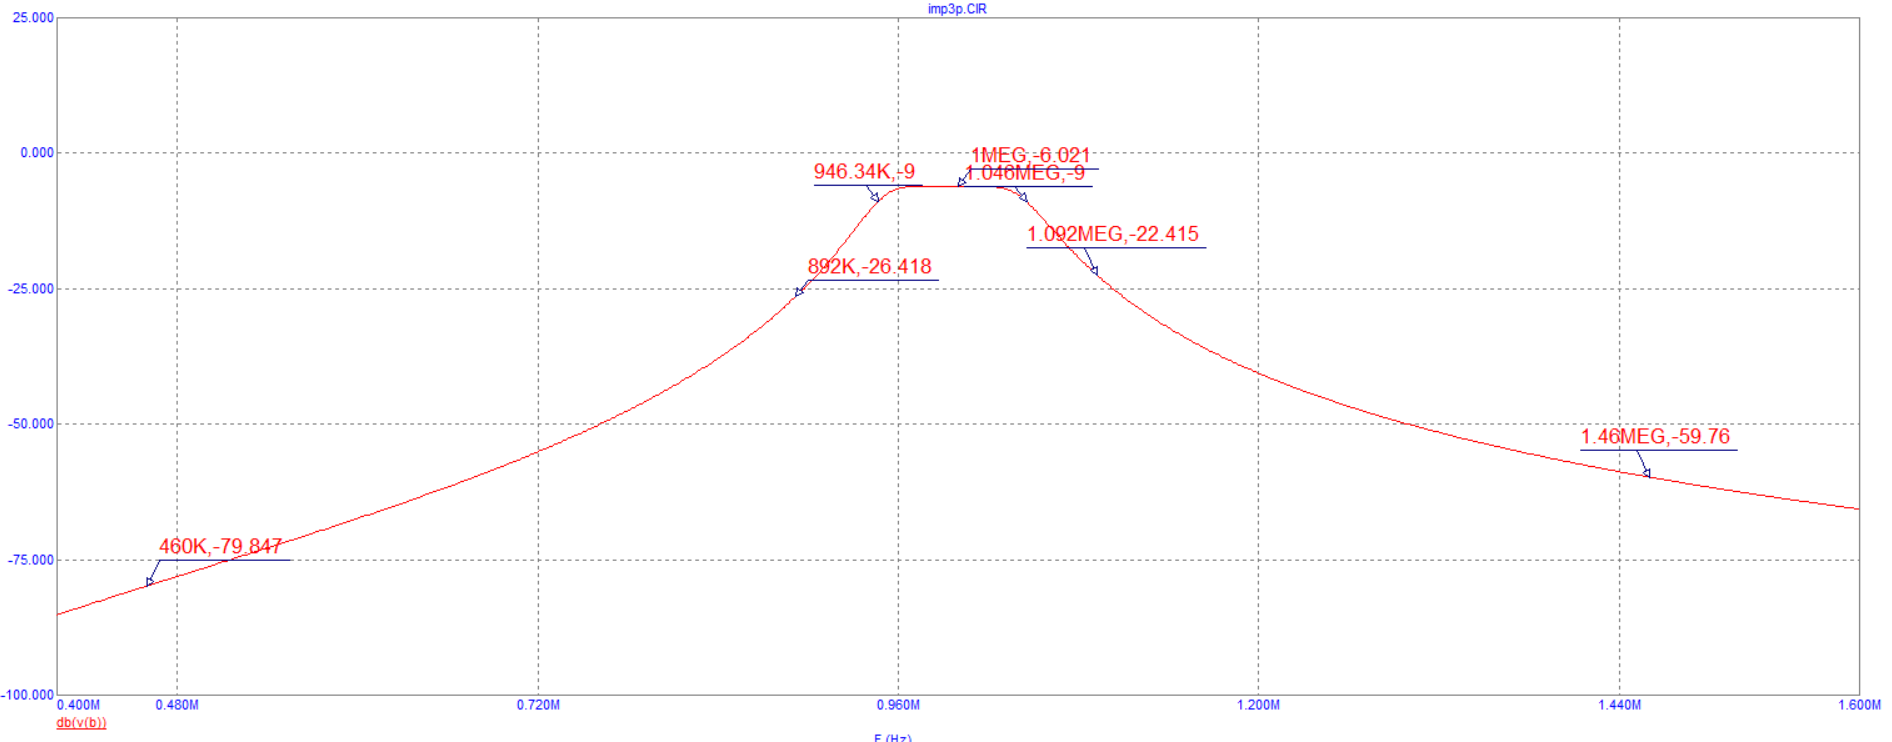
\includegraphics[width=1.0\linewidth]{res/imp3p_bandpass_log.png}
		\caption{ПФ, затухание}
		\label{phase}
	\end{figure}

	\subsubsection*{7}
	
	Наконец, рассмотрим режекторный фильтр. Измерим ширины полос режекции на заданных уровнях.
	\begin{figure}[H]
		\centering
		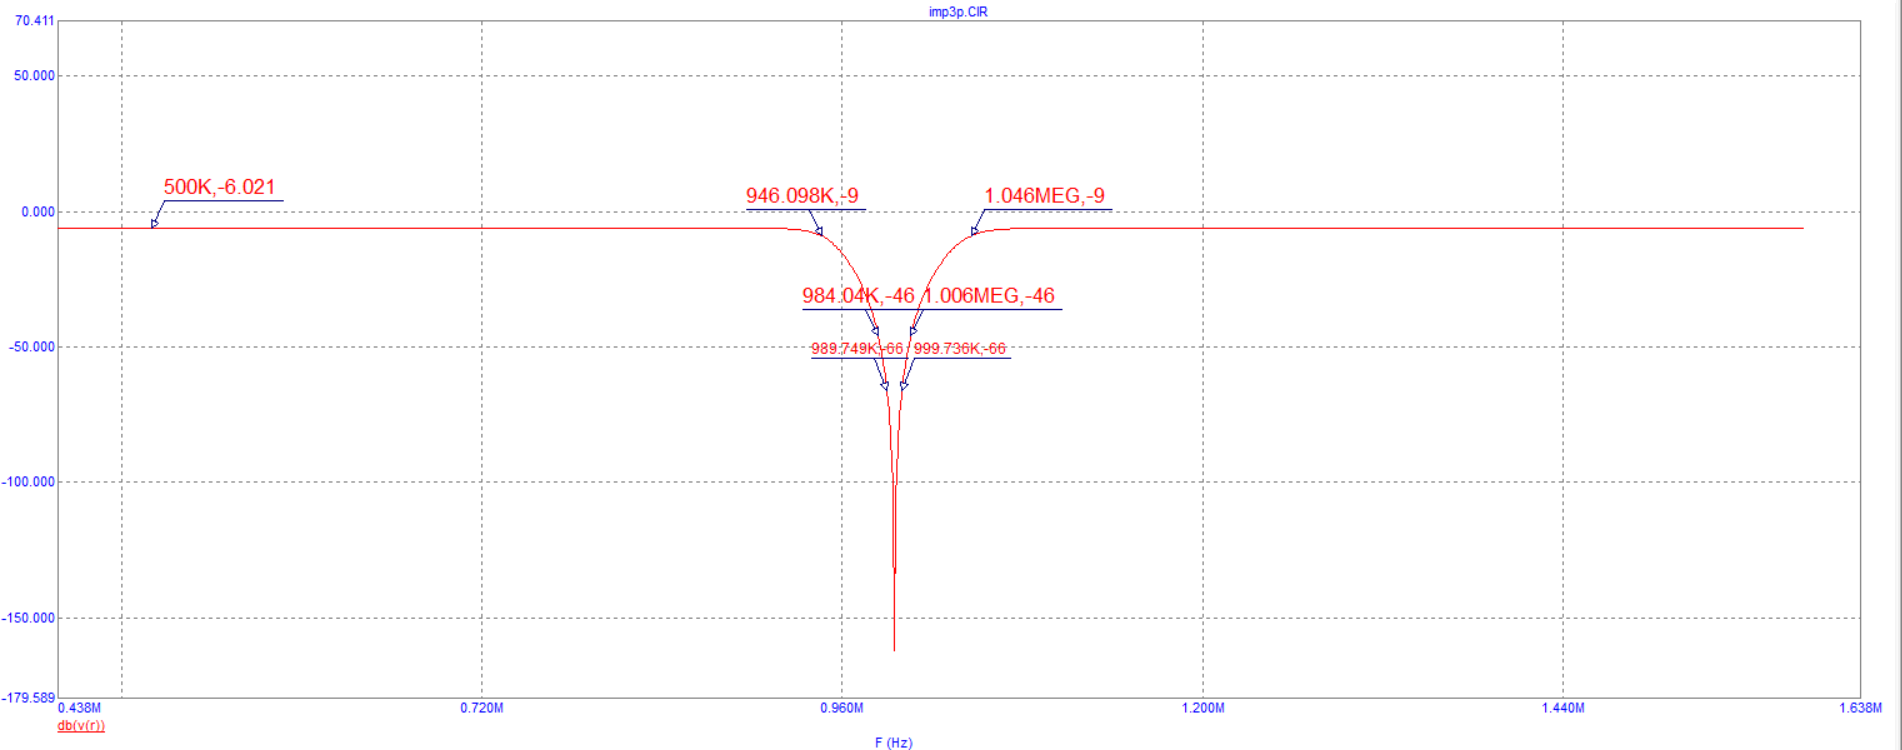
\includegraphics[width=1.0\linewidth]{res/imp3p_reject_log.png}
		\caption{РФ, затухание}
		\label{phase}
	\end{figure}

	\begin{table}[H]
		\begin{tabular}{llll}
			\hline
			Затухание  & $-3 \; dB$ & $-43 \; dB$ & $-63 \; dB$ \\ \hline
			$\Delta f$ & $100 \; k$ & $22 \; k$   & $10 \; k$   \\ \hline
		\end{tabular}
		\caption{Ширина полосы от уровня затухания}
	\end{table}	
		
	\subsection*{9.3 Фильтры нижних частот высших порядков}
	
	Рассмотрим графики ФНЧ Баттерворта с различным числом полюсов. Приведем значения затухания.
	\begin{figure}[H]
		\centering
		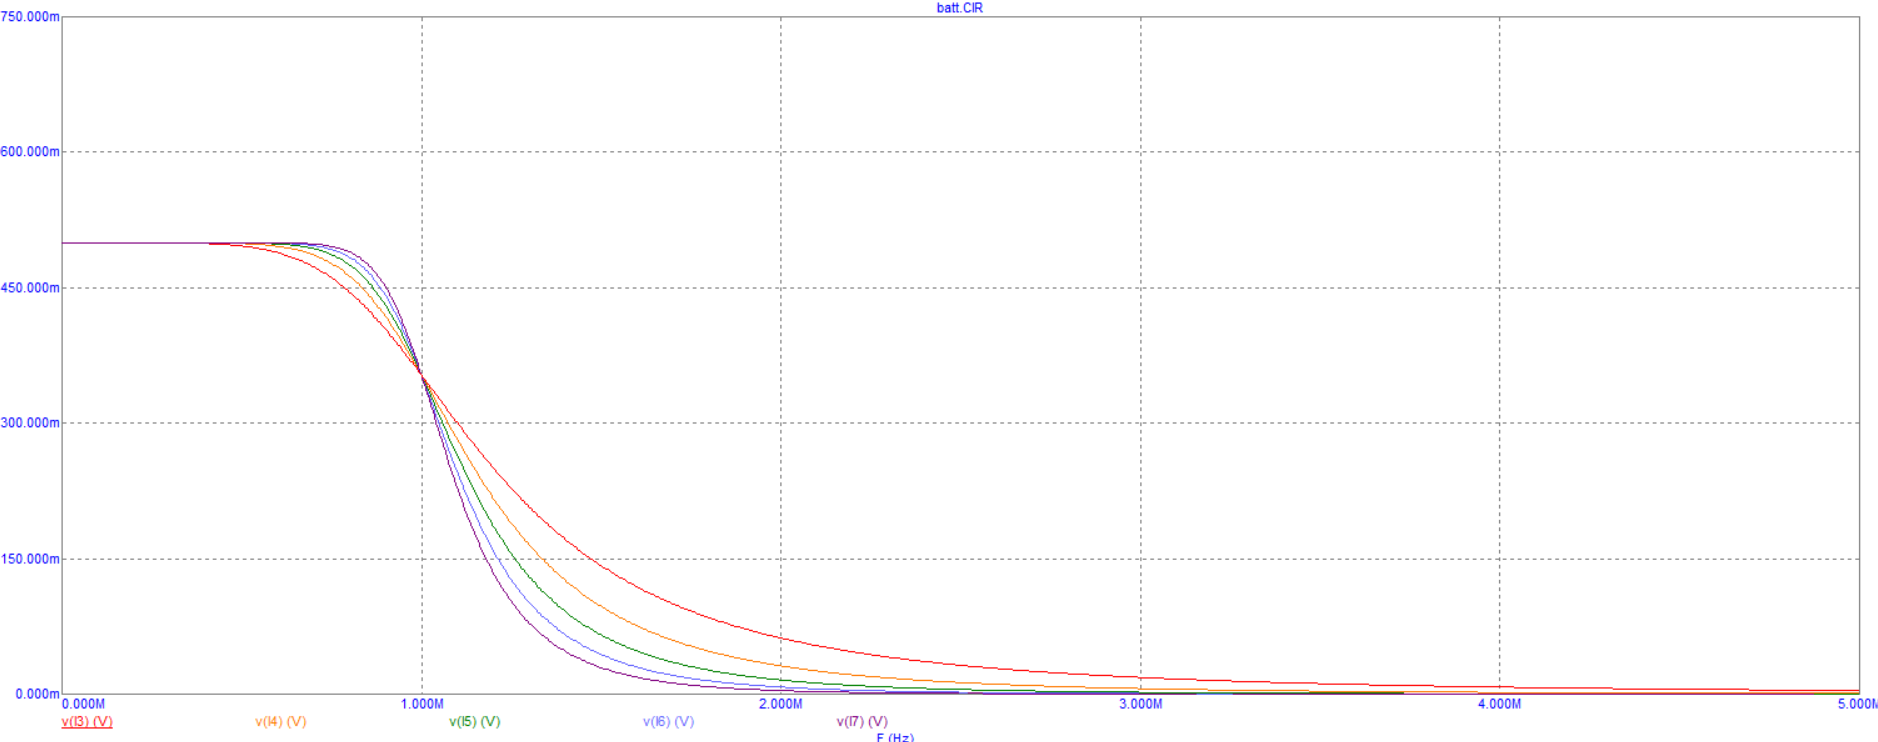
\includegraphics[width=1.0\linewidth]{res/batt.png}
		\caption{ФНЧ Баттерворта высших порядков}
		\label{phase}
	\end{figure}
		
	\begin{table}[H]
		\begin{tabular}{llll}
			\hline
			$n \backslash f$ & $f_0$ & $2f_0$ & $10f_0$ \\ \hline
			3     & -3    & -18    & -60     \\
			4     & -3    & -24    & -80     \\
			5     & -3    & -30    & -100    \\
			6     & -3    & -36    & -120    \\
			7     & -3    & -42    & -140    \\ \hline
		\end{tabular}
		\caption{Уровни затухания ФНЧ Баттерворта от порядка фильтра}
	\end{table}

	Проведем те же измерения для фильтров Чебышева с неравномерностью $0.5 \; dB$ и $3.0 \; dB$.
	\begin{figure}[H]
		\centering
		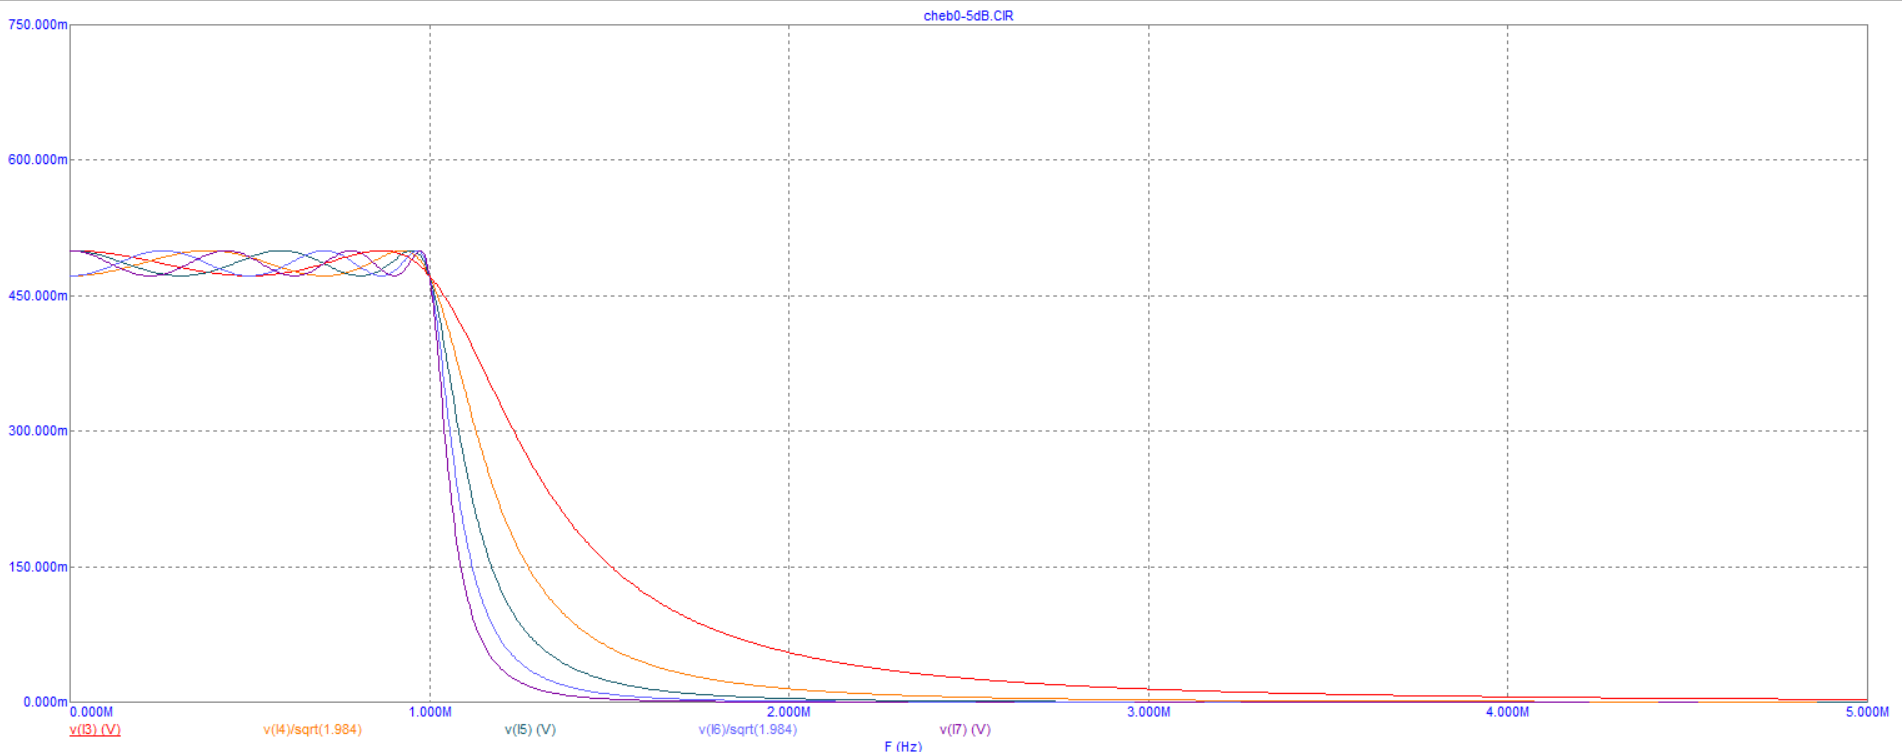
\includegraphics[width=1.0\linewidth]{res/cheb05.png}
		\caption{ФНЧ Чебышева, неравномерность = $0.5$ dB}
		\label{phase}
	\end{figure}
	
	\begin{figure}[H]
		\centering
		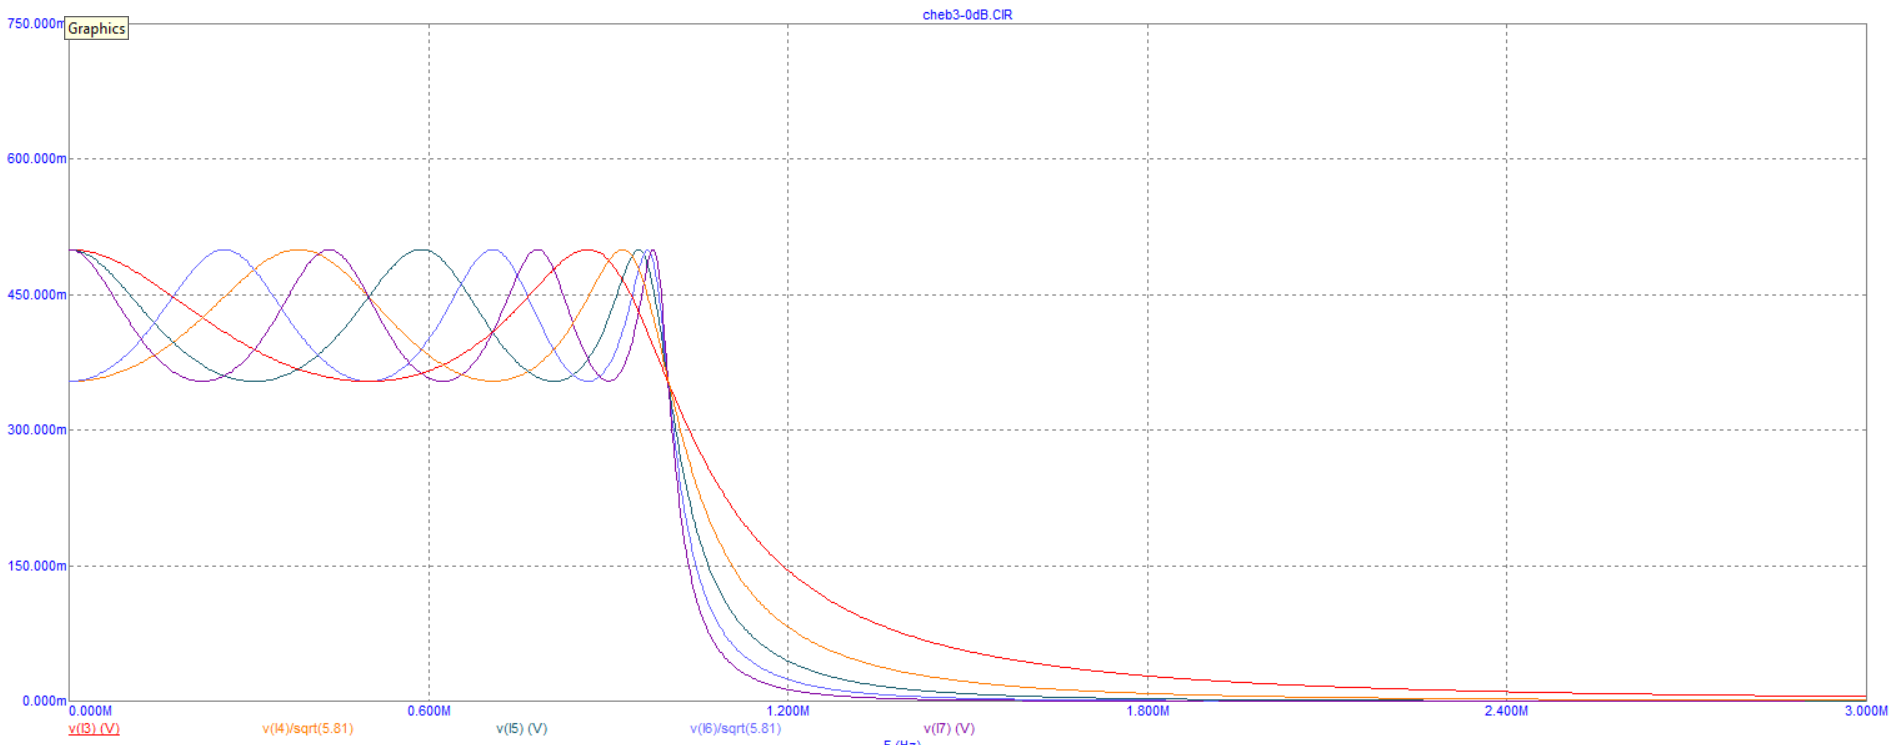
\includegraphics[width=1.0\linewidth]{res/cheb3.png}
		\caption{ФНЧ Чебышева, неравномерность = $3.0$ dB}
		\label{phase}
	\end{figure}

	Составим таблицы затуханий для всех трех фильтров на частотах $f = 2f_0$ и $f = 10 f_0$.

	\begin{table}[H]
		\begin{tabular}{llllll}
			\hline
			$n$                   & 3   & 4   & 5   & 6   & 7   \\ \hline
			Баттерворт            & -18 & -24 & -30 & -36 & -42 \\
			Чебышев $(0.5 \; dB)$ & -19 & -30 & -42 & -53 & -64 \\
			Чебышев $(3.0 \; dB)$ & -28 & -39 & -51 & -62 & -74 \\ \hline
		\end{tabular}
		\caption{Неравномерности ФНЧ, $f=2 f_0$}
	\end{table}

	\begin{table}[H]
		\begin{tabular}{llllll}
			\hline
			$n$                   & 3   & 4   & 5    & 6    & 7    \\ \hline
			Баттерворт            & -60 & -80 & -100 & -120 & -140 \\
			Чебышев $(0.5 \; dB)$ & -62 & -88 & -114 & -140 & -166 \\
			Чебышев $(3.0 \; dB)$ & -71 & -98 & -123 & -149 & -175 \\ \hline
		\end{tabular}
		\caption{Неравномерности ФНЧ, $f=10 f_0$}
	\end{table}


	\subsection*{9.4 Фильтры пятого порядка}
	
	Нормализуем фильтры к фильтрам Баттерворта. Аналогично нормализуем к фильтрам Чебышева с неравномерностью $0.5 \; dB$ и $3.0 \; dB$.
	
	Настроим фильтры на $Q = 5, \; R_0 = 50, \; f_0 = 1 \; MHz$.
	
	Сделана в MicroCap.
	
	
	\subsection*{9.5 Семиполюсной фильтр}

	Нормализуем семиполюсной фильтр к ПФ Баттерворта и ПФ Чебышева с неравномерностью $0.5 \; dB$ и $3.0 \; dB$.

	Настроим фильтры на $Q = 19.375, \; R_0 = 600, \; f_0 = 465 \; kHz, \Delta f = 24 \; kHz$.

	\begin{figure}[H]
		\centering
		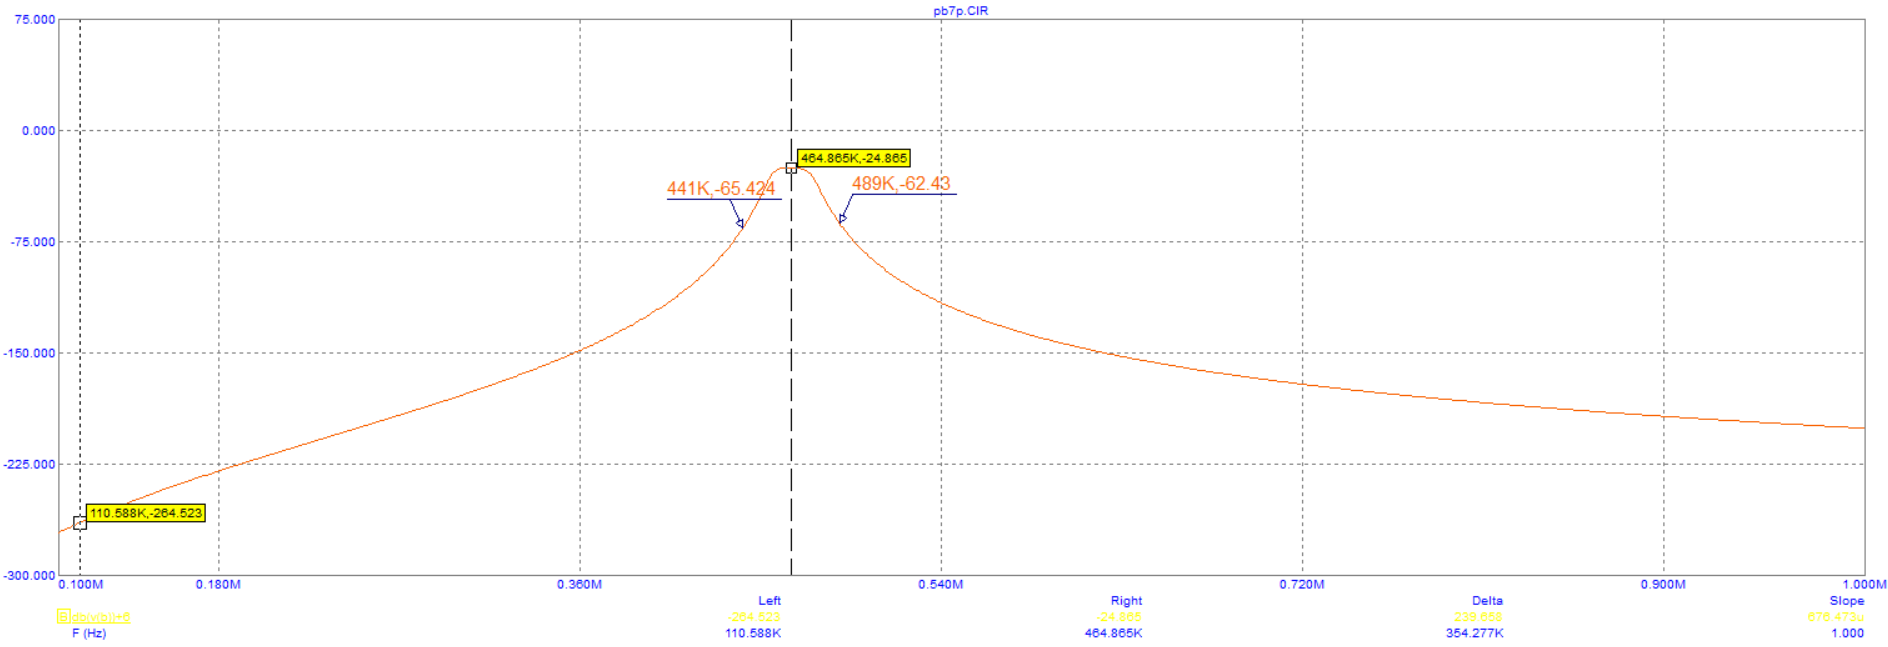
\includegraphics[width=1.0\linewidth]{res/pb7p_batt.png}
		\caption{ПФ Баттерворта}
		\label{phase}
	\end{figure}
	
	\begin{figure}[H]
		\centering
		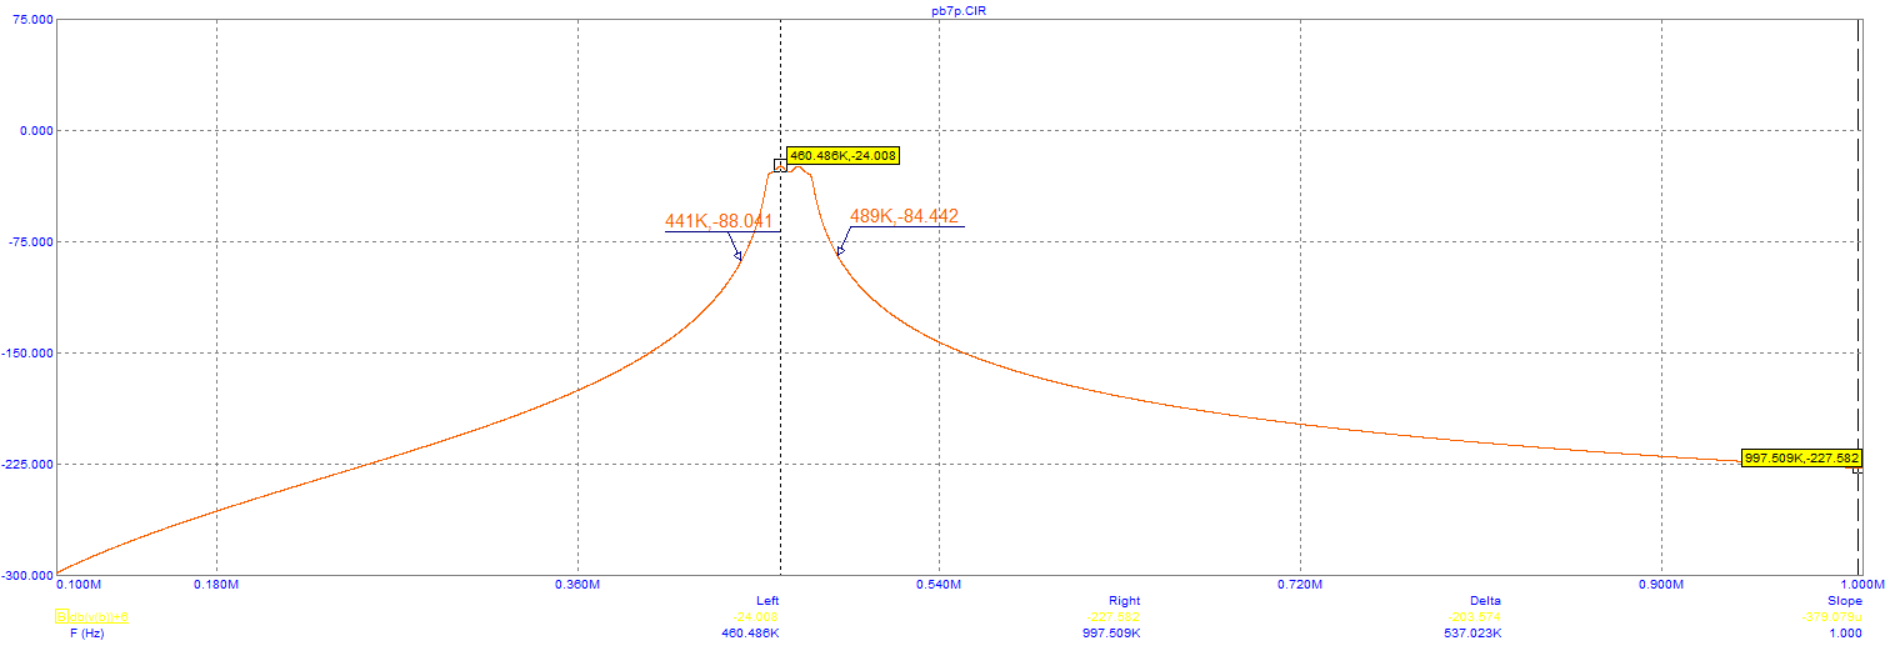
\includegraphics[width=1.0\linewidth]{res/pb7p_cheb05.png}
		\caption{ПФ Чебышева, неравномерность = $0.5$ dB}
		\label{phase}
	\end{figure}
	
	
	\begin{figure}[H]
		\centering
		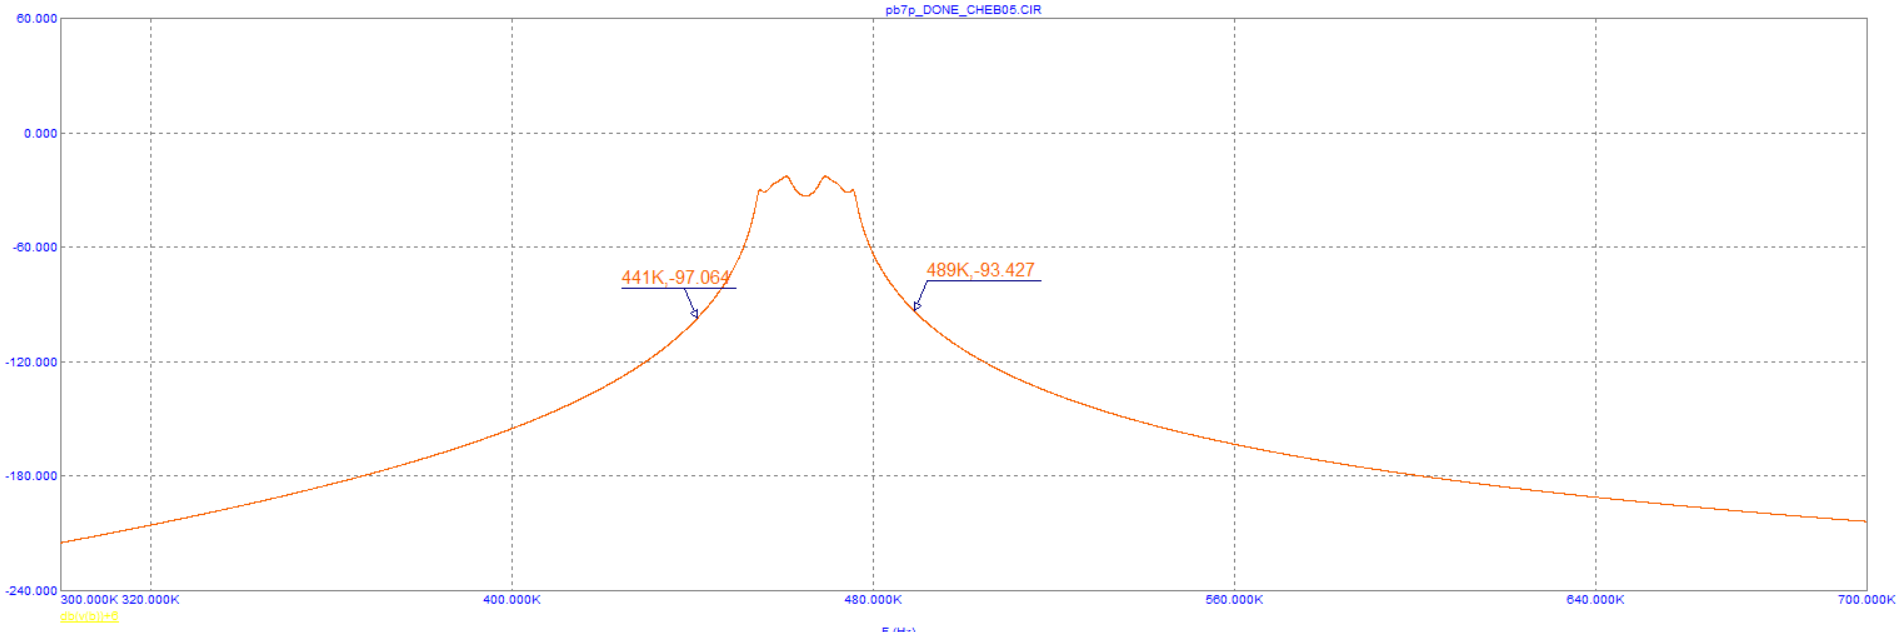
\includegraphics[width=1.0\linewidth]{res/pb7p_cheb3.png}
		\caption{ПФ Чебышева, неравномерность = $3.0$ dB}
		\label{phase}
	\end{figure}
		
\end{document}